\chapter[Fundamentação Teórica]{Fundamentação Teórica}

O estudo de Inteligência Artificial vem sendo cada vez mais comum na comunidade de tecnologia da informação para a criação de sistemas que buscam automatizar e auxiliar de maneira mais eficiente o trabalho humano. O presente capítulo traz a explicação de um conjunto de tecnologias da área de IA para que seja possível contextualizar o leitor sobre o tema abordado no presente trabalho \hl{MELHORAR DESCR}.

\section{Aprendizagem de Máquina}

Aprendizado de Máquina do inglês \textit{Machine Learning} (ML) é uma das subáreas da Inteligência Artificial que visa criar mecanismos que possibilitem fazer com que uma máquina possa "aprender" sobre um determinado problema a partir de um conjunto de dados de entrada. Em outras palavras, ML permite que um dado algoritmo desenvolva uma função matemática que consiga representar tal conjunto de dados. Com essa função ou modelo matemático, é possível agora realizar inferências sobre outros dados, desde que esses sejam relacionados à mesma problemática \cite{deep-learning-book-br}.

O processo de aprendizagem se da início a partir de observações ou dados, como exemplos, experiência direta ou instruções que possibilitem identificar padrões do dado para realizar e atingir melhores decisões em futuras apresentações ou exemplos de dados que possam ser fornecidas. Dentro do processo de permitir que uma máquina aprenda, existem três áreas as quais os mecanismos de aprendizagem são classificados \cite{python-ml}:

\begin{itemize}
  \item \textbf{Aprendizado supervisionado:} o objetivo principal de algoritmos supervisionados é conseguir desenvolver um modelo matemático a partir de um conjunto de dados anotados, no caso, dados de treinamento. O \textit{supervisionado} diz respeito ao conjunto de dados os quais já se sabe a saída esperada, ou seja, o dado já é anotado previamente. Em geral, esses algoritmos são utilizados para problemas de classificação e regressão.

  % fonte: https://blogs.nvidia.com/blog/2018/08/02/supervised-unsupervised-learning/

  \begin{figure}
    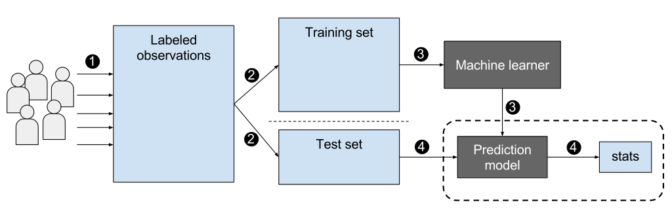
\includegraphics[width=\linewidth]{figuras/nvidia-supervised-learning.png}
    \caption{Aprendizado supervisionado \hl{OBS: COLOCAR FONTE}}
    \label{fig:nvidia-supervised-learning}
  \end{figure}
  \newpage
  \item \textbf{Aprendizado não supervisionado:} diz respeito aos métodos de aprendizagem de máquina os quais utiliza-se como dado de entrada um dado que não possui nenhum tipo de anotação e que, muitas vezes, sua estrutura é desconhecida.

  Tal processo de aprendizagem permite extrair características relevantes sobre o dado que possam servir de insumo para uma futura categorização e classificação do mesmo. Dependendo do problema em questão, a aprendizagem supervisionada pode organizar o dado em diferentes categorias \cite{learning-types} como clusterização, associação, \textit{autoencoders}, \textit{anomaly detection}, etc.

  \item \textbf{Aprendizado semi-supervisionado:} já o aprendizado semi-supervisionado junta um pouco dos dois mundos: dados com registros anotados e também dados com registros não anotados. A aplicabilidade para esse tipo de aprendizagem é quando se possui um dado onde não é trivial extrair informações relevantes sobre ele e tampouco é realizar toda a anotação da amostra em questão \cite{learning-types}.
\end{itemize}

Dentro dos tipos de algoritmos que podem ser utilizados para construir ML, geralmente em aprendizagem supervisoonada e semi-supervisionada, um que é bastante notado se não o mais conhecido são as chamadas Redes Neurais Artificiais ou \textit{Neural Networks} (NN). Diferentemente de \textit{Machine Learning} convencional, as NN é um campo dentro de ML que possiblita o aprendizado de máquina tentando imitar o comportamento dos neurônios humanos \cite{neural-net-history} e está associado diretamente ao \textit{Deep Learning}.

\subsection{\textit{Neural Networks}}

Em 1943, Warren McCullock e Walter Pitts em seu artigo \textit{A Logical Calculus of the Ideas Immanent in Nervous Activity} desenvolveram um estudo para tentar explicar como o cérebro consegue reconhecer um nível complexo de padrões por meio dos neurônios \cite{first-neuron-study}, desenvolvendo um modelo chamado MCP (McCullock-Pitts) que atualmente é conhecido como o ancestral das redes neurais artificiais \cite{dl-brief-review}. Tal estudo possibilitou dar-se o pontapé para a evolução das redes neurais que conhecemos hoje.

Na década de 1950 surgiu então o modelo de \textit{Perceptron} \cite{perceptron}, que é a primeira rede neural formalmente desenvolvida composta de apenas uma única camada, descrito como um modelo matemático que recebe várias entradas e produz uma saída binária.

% fonte da imagem: https://towardsdatascience.com/the-perceptron-3af34c84838c

\begin{figure}[h]
  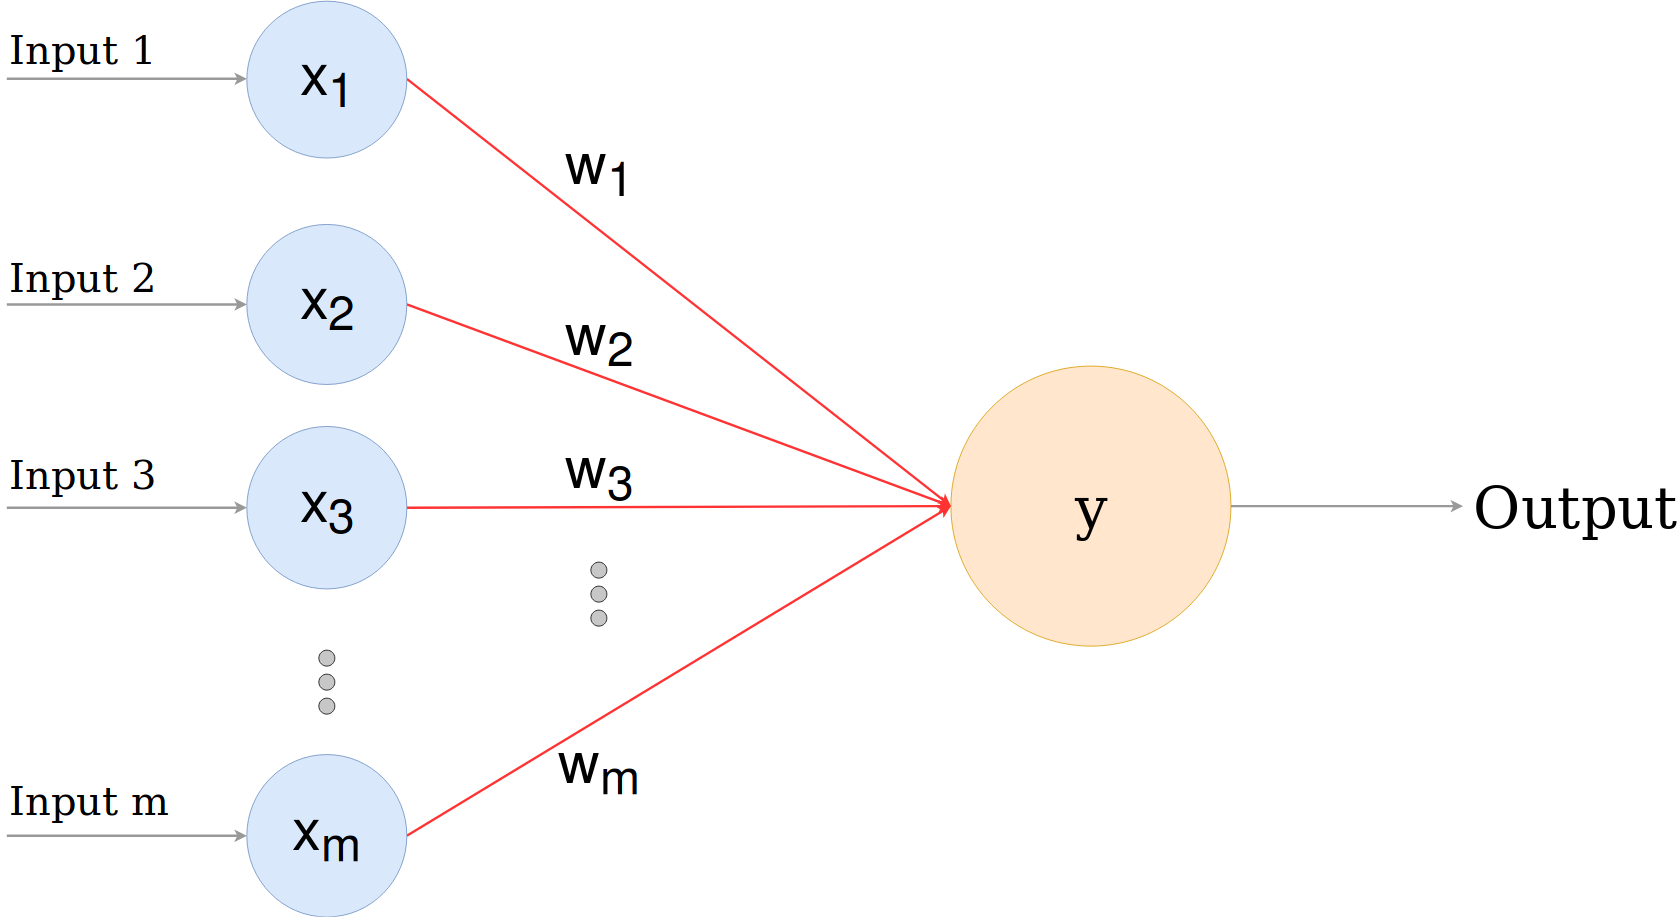
\includegraphics[width=13cm, center]{figuras/perceptron}
  \caption{O \textit{Perceptron} \hl{OBS: COLOCAR FONTE}}
  \label{fig:perceptron}
\end{figure}

Cada entrada ou \textit{input} representa um dado de entrada que é inserido diretamente nos nós de entrada ou \textit{input nodes}, representados pela letra \(x\). Cada um desses nós representam separadamente uma característica do dado de entrada. Na figura \ref{fig:perceptron}, a quantidade de características é delimitada pela letra \(m\) e o intervalo de características é dado por [1, \(m\)]. A camada caracterizada pelas letras \textit{x} é chamada de camada de entrada ou \textit{input layer}. Redes Neurais só podem receber como entrada valores numéricos \cite{deep-learning-book-br}.

É importante reparar na figura \ref{fig:perceptron} que todo nó da camada de entrada está diretamente associado com uma seta caracterizada pela letra \(w\), também de intervalo [1, \(m\)]. Tais letras caracterizam o que é conhecido como os pesos ou \textit{weights}. As setas são chamadas de sinapses\footnote
{
  Na biologia, sinapse é a região localizada entre os neurônios e agem como neurotransmissores, responsáveis por realizar a transferência de inpulso nervoso de um neurônio para o outro \cite{synapses}.
}.
Essa região é definida como camada de pesos ou \textit{weight layer}.

Por fim, tem-se o nó de maior tamanho definido pela letra \(y\), conhecido como nó de saída ou \textit{output node}. Esse nó realiza um cálculo baseado em \textit{score} sobre os valores de entrada e peso e por meio de uma função de ativação, gera uma predição \textit{output} de 0 ou 1 sobre o valor resultante do \textit{score}.

A função matemática que define o valor encontrado em \(y\) é:

\[ y = f(x) = \sum_{i=1}^{m} x_iw_i + B\]

onde a função de ativação consome o valor resultante da função \(f(x)\), que serão melhor detalhadas na seção \ref{sssec:activation-func}. \(B\) na função define o \textit{bias} ou erro, adicionado ao valor resultante da soma de multiplicações para possíveis correções. O termo \textit{bias} foi introduzido por Tom M. Mitchell em seu artigo \textit{The Need for Biases in Learning Generalizations} \cite{biases} e o objetivo dele é possibilitar que o modelo generalize melhor o problema e seja menos sensível ao dado de entrada.

\subsubsection{Função de Ativação} \label{sssec:activation-func}

Funções de ativação são funções matemáticas que determinam o resultado de uma saída \textbf{\(z\)} de um neurônio em uma rede neural, baseando-se em um \textit{threshold}\footnote{
  o que é threshold
} \textbf{\(t\)} \hl{COLOCAR DEFINICAO}.
A partir do valor resultante \textbf{\(y\)} da soma dos valores de entrada \(x_i\) multiplicados pelos pesos \(w_i\) dentro do intervalo \([1, m]\) definido na fórmula \hl{COLOCAR REF}, se esse valor alcança ou ultrapassa o \textit{threshold}, o neurônio é ativado. Caso não alcante, ele não é ativado e seu sinal não é propagado \cite{python-ml}.

\[
  z =
  \begin{cases}
    1, & \text{se } y\geq \textit{t} \\
    0, & \text{se } y < \textit{t}
  \end{cases}
\]

A função principal das funções de ativação dentro de uma rede neural é adicionar a não-linearidade ao problema, permitindo assim que tais redes consigam computar problemas não triviais \cite{gentle-intro-to-nn}. Os principais problemas que envolvem ML, principalmente no âmbito da computação visual - foco do presente trabalho -, a porcentagem de problemas que a solução é resolvida por meio de uma equação linear é praticamente - se não - zero.

Existem diversos tipos de funções de ativação com aplicabilidade em diversos tipos de problemáticas a serem resolvidas. A figura \ref{fig:activation-functions} lista as principais e mais conhecidas funções de ativação, sendo que pesquisadores ainda realizam estudos para encontrar funções que apresentem melhores resultados \cite{intro-to-act-func}.

% fonte: https://medium.com/@shrutijadon10104776/survey-on-activation-functions-for-deep-learning-9689331ba092

\begin{figure}[H]
  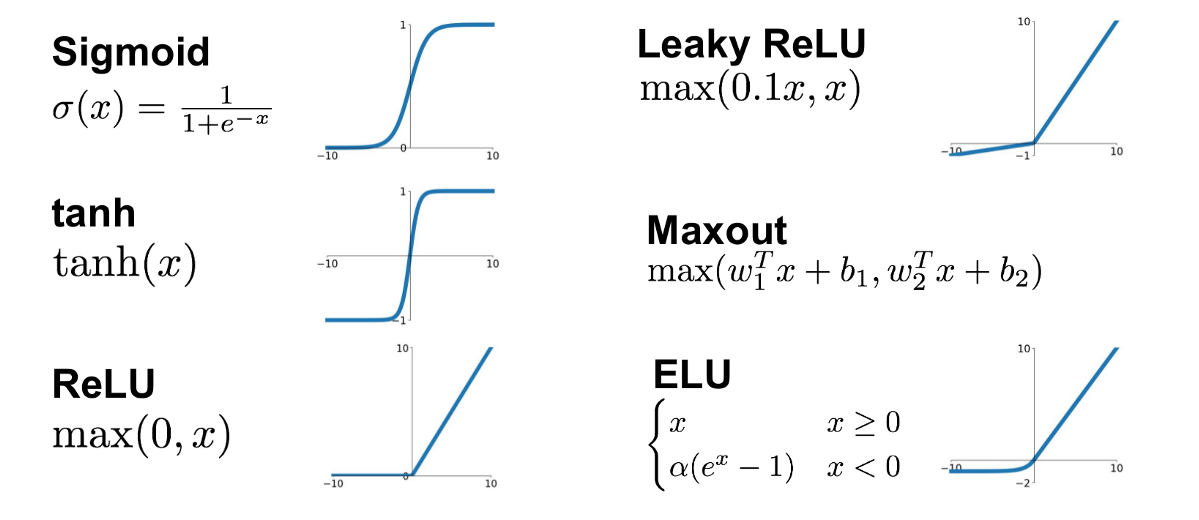
\includegraphics[width=12cm, center]{figuras/activation-functions}
  \caption{Principais funções de atiação \hl{OBS: COLOCAR FONTE}}
  \label{fig:activation-functions}
\end{figure}

É importante ressaltar que um único \textit{Perceptron} não é capaz de solucionar problemas não-lineares. Algoritmos que possibilitam solucionar problemas não-lineares serão descritos na seção \ref{sssec:cnn}, detalhando um pouco da evolução dos algoritmos para algo mais conhecido atualmente.

\subsubsection{\textit{Weights}}

Os pesos representam o grau de conexão entre dois neurônios distintos. Por exemplo: se o peso de um neurônio 1 para o neurônio 2 tem uma maior magnitude, significa que o neurônio 1 tem maior importância sobre o neurônio 2.

Em termos práticos, o peso consegue definir o quão relevante para o problema aquele determinado valor de entrada é. Pesos que se aproximam de zero tendem a diminuir a importância do valor de entrada para o valor resultante da rede \cite{everything-about-nn}.

\subsubsection{Redes Neurais Convolucionais} \label{sssec:cnn}

Conhecendo melhor o \textit{Perceptron} e entendendo como ele funciona, é possível identificar da sua limitação: a linearidade. Para solucioar esse problema, adiciona-se uma função de ativação para cada valor resultante de um nó e coloca-se esses nós em contato com mais nós de uma outra camada, adicionando assim mais camadas de processamento e identificação de características dos dados. As redes de camadas multiplas de nós ou \textit{perceptrons} é chamada de \textit{Multilayer Perceptrons} ou MLP \cite{deep-learning-book-br}.

O conjunto de de novas camadas, sendo essas diferentes da \textit{input} e \textit{output layers}, são chamadas de camadas ocultas ou \textit{hidden layers} \cite{goodfellow-et-al-2016}. A definiçãode \textit{Deep Learning} se dá pela quantidade de camadas ocultas na arquitetura da sua rede neural, sendo a MLP a "\textit{Hello World}" das arquiteturas de RNAs.

Mais tarde, em 1998, os pesquisadores Yann LeCun, Leon Bottou, Yosuha Bengio e Patrick Haffner desenvolveram uma nova arquitetura de rede neural herdando as características já existentes no MLP, como propagação de sinal ou \textit{forward pass} (seção \ref{sssec:forward-pass}), \textit{backpropagation} (seção \ref{sssec:backpropagation}), taxa de aprendizagem (seção \ref{sssec:learning-rate}), entre outros. Tal arquitetura foi chamada de LeNet-5 \cite{le-net} e sua função era conseguir reconhecer dígitos manuscritos de 0 à 9. Os dados utilizados para o experimento é chamado de \href{http://yann.lecun.com/exdb/mnist/}{MNIST}. Essa nova arquitetura evoluiu para o que conhecemos hoje como Redes Neurais Convolucionais ou CNN (\textit{Convolutional Neural Networks}) \cite{goodfellow-et-al-2016}.

\begin{figure}[H]
  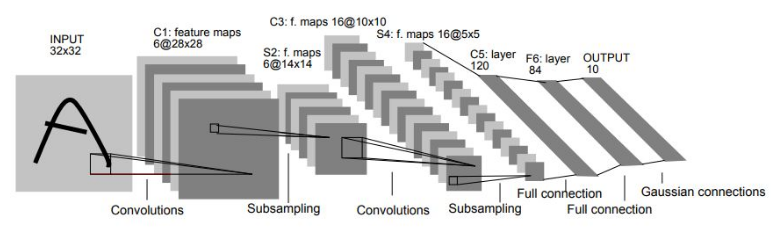
\includegraphics[width=\linewidth]{figuras/le-net.png}
  \caption{Arquitetura da LeNet-5 \hl{OBS: COLOCAR FONTE}}
  \label{fig:le-net}
\end{figure}

As CNNs são redes neurais especializadas em dados mais complexos, principalmente para lidar com dados de imagens \cite{goodfellow-et-al-2016}. A função da CNNs em relação a visão computacional é tentar reduzir a dimensionalidade das imagens para que o seu processamento seja mais simples, mantendo as características críticas para uma boa predição \cite{comprehensive-guide-to-cvv}.

Diferentemente das redes neurais convencionais como a MLP, as CNNs utilizam da convolução como forma de cálcular os valores dos neurons em um ou mais camadas, ao invés de utilizar cálculo matricial convencional \cite{goodfellow-et-al-2016}, e por isso herdam em seu nome a palavra \textbf{convolução}. Além disso, as CNNs utilizam possuem também, além de camadas de convolução (sessão \ref{ssssec:convolution}), camadas de \textit{pooling} (sessão \ref{ssssec:pooling}) e totalmente conextadas ou \textit{fully-connected layer} (sessão \ref{ssssec:fully-connected}).


\subsubsubsection{Convolução} \label{ssssec:convolution}
Na matemática, a convolução é uma operação sobre duas funções que operam com números reais (\(f\) e \(g\)) que gera uma terceira função (\(z\)) a qual expressa como uma função tende a afetar ou moldar o formato da outra. Ela representa a integral do produto de duas funções depois que uma delas foi alterada ou movida.

\[
  z(t) = \int f(a)g(t - a) da
\]

Essa é a função matemática que define a \textbf{convolução}. Para simplificação, a convolução é traduzida utilizando o símbolo de asterisco.

\[
  z(t) = (f * g)(t)
\]

Com um olhar para as redes neurais convolucionais, o primeiro argumento da convolução (\(f\)) se refere aos dados de entrada ou \textit{inputs}. O segundo argumento (\(g\)) é denominado \textit{kernel}. O resultado (\(z\)) costuma ser referenciado como mapa de características ou \textit{feature map}. É importante ressaltar que nas CNNs, os dados presentes tanto no \textit{input} quanto os dados do \textit{kernel} devem ser números inteiros, pois trabalha-se a convolução discreta no processo matemático \cite{goodfellow-et-al-2016}.

Em aplicações de ML, o \textit{input} é geralmente tratado como um vetor multidimensional de dados e o \textit{kernel} é um vetor multidimensional de parâmetros, o qual é adaptado a medida que o processo de aprendizado corrige tais parâmetros para melhorar os resultados e minimizar a função de custo (\textit{cost function}). A função de correção dos parâmetros é chamada de \textit{backpropagation} e será tratada na sessão \ref{sssec:backpropagation}. A função de custo será tratada na sessão \ref{sssec:cost-function}.

Na prática, é possível então implementar essa integral como sendo a somatória dentro de um intervalo finito das dimensões desses vetores mutidimensionais (também chamados de tensores). Em geral, combina-se a convolução em mais de um eixo por vez sem realizar nenhum giro ou modificação em nenhuma das funções, chamando-a de correlação cruzada ou \textit{cross-relation} \cite{goodfellow-et-al-2016}, permitindo assim:

\[
  z(i, j) = (I * K)(i, j) = \sum_{m} \sum_{n} I(i + m, j + n)K(m,n)
\]

Na equação acima \hl{COLOCAR REF} o \(I\) representa o tensor de entrada, \(K\) o tensor de \textit{kernel}, \(i\) e \(j\) a largura e altura do tensor de entrada, respectivamente, E \(m\) e \(n\) a largura e algura do tensor \textit{kernel}, respectivamente.

% a good one: https://mlnotebook.github.io/post/CNN1/
% fonte: https://medium.com/machine-learning-for-li/different-convolutional-layers-43dc146f4d0e
\begin{figure}[H]
  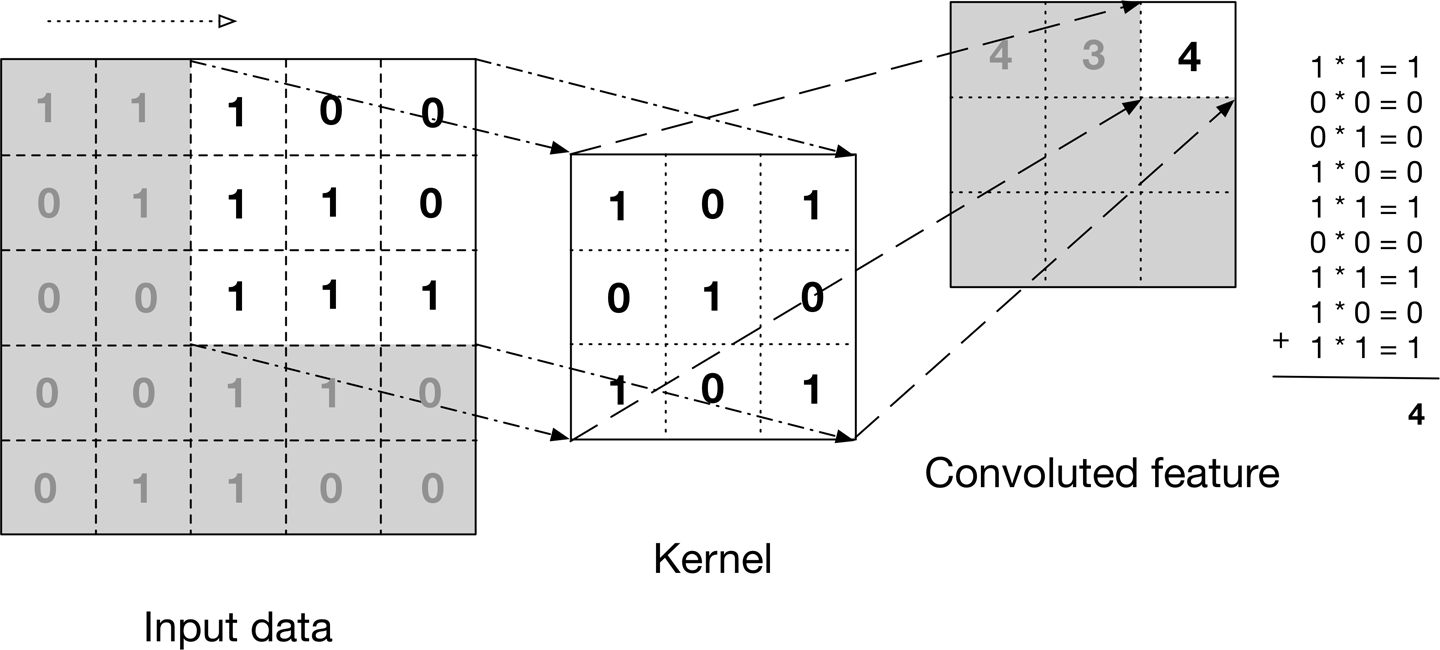
\includegraphics[width=\linewidth]{figuras/cnn-kernel-multiplication.png}
  \caption{Camada de convolução. \hl{OBS: COLOCAR FONTE}}
  \label{fig:cnn-kernel-multiplication}
\end{figure}

Existem uma série de parâmetros que podem ser utilizados para a configuração do algoritmo de convolução de uma Rede Neural Convolucional. Tais parâmetros, geralmente citados como hiperparãmetros, serão explicados de maneira geral na sessão \ref{sssec:hiperparameters}. O conjunto de hiperparâmetros para as CNNs, como \textit{depth}, \textit{stride}, tamanho do kernel, etc estarão melhor descritos no apêndice \hl{CRIAR APENDICE PARA REFERENCIAR}.

\subsubsubsection{\textit{Pooling}} \label{ssssec:pooling}
\subsubsubsection{\textit{Fully-connected Layer}} \label{ssssec:fully-connected}

\subsubsection{\textit{Propagação de sinal}} \label{sssec:forward-pass}

\subsubsection{\textit{Backpropagation}} \label{sssec:backpropagation}

\subsubsection{\textit{Função de custo}} \label{sssec:cost-function}

\subsubsection{\textit{Taxa de aprendizagem}} \label{sssec:learning-rate}

\subsubsection{Hiperparâmetros} \label{sssec:hiperparameters}


\subsection{Discriminativo vs Generativo}

\section{OCR}